\documentclass[]{article}
\usepackage{polski}
\usepackage{graphicx}
\usepackage{xcolor}
\usepackage{subcaption}
\usepackage{geometry}
\usepackage{ragged2e}
\usepackage{amsthm}
\usepackage{amsmath}
\usepackage{amssymb}
\usepackage{titlesec}
\usepackage{float}
\usepackage{etoolbox}
\usepackage{hyperref}
\geometry{
	a4paper,
	left=2.5cm,
	right=2.5cm,
	top=3cm,
	bottom=3cm}
	\titleformat{\section}[hang]{\LARGE\bfseries\raggedright}{\thesection}{0.5cm}{}
	\titleformat{\subsection}[hang]{\large\bfseries\raggedright}{\thesubsection}{0.5cm}{}
	
\begin{document}
	

	
\begin{center}
\centering
\vspace*{2cm}

\textbf{\Huge  POLITECHNIKA LUBELSKA} \\
\vspace{0.5cm}
\textbf{\LARGE WYDZIAŁ MATEMATYKI I} \\
\vspace{0.5cm}
\textbf{\LARGE INFORMATYKI TECHNICZNEJ}\\
\vspace{1cm}

\textit{Kierunek:} Inżynieria i Analiza Danych \\




\end{center}


		\begin{figure}[h]
			
\includegraphics[width=0.4\textwidth]{logo_politechniki.png}
			\label{}
			\centering
		\end{figure}
		\begin{figure}[h]
			
\includegraphics[width=0.4\textwidth]{logo_wydziału}
			\label{}
			\centering
		\end{figure}
		\centering
		\textbf{Narzędzia informatyczne II}\\
		\vspace{0.5cm}
		\centering
		\textbf{Projekt zaliczeniowy MATLAB}\\
		\vspace{0.5cm}


	\textit{Wykonały:} \textbf{ Maja D,  Weronika K}

\newpage

\section*{\textbf{\Huge Dowolne ciągi zbieżne}}

\tableofcontents
\section{Podstawowe pojęcia}
\subsection{Definicja ciągu}

\label{sec:pierwsza}
\newtheorem*{df}{\textcolor{red}{DEFINICJA}}
\newtheorem*{tw}{\textcolor{blue}{TWIERDZENIE}}
	\begin{df}
	
	 \cite{label1} Ciągiem liczbowym nazywamy funkcję $a : \mathbb{N} \to \mathbb{R}$  odwzorowującą zbiór liczb naturalnych $\mathbb{N}$ w zbiór liczb rzeczywistych $\mathbb{R}$ i oznaczamy przez {$a_n$}. Używamy zapisu \\
	 \begin{equation*}
	 	\centering
	 	a_n=a(n).
	 \end{equation*}
	Ciąg ${a_n}$ można też zapisywać w postaci \\
	\begin{equation*}
		\centering
		 a_1, a_2, a_3, ..., a_n, ...
	\end{equation*}
	 Liczbę $a_n$ nazywamy n-tym wyrazem ciągu ${a_n}$.
	\end{df}


		



\subsection{Monotoniczność i ograniczoność ciągu liczbowego}
\label{sec:druga}
\begin{tw}
	Mówimy, że ciąg $a_n$ jest: 
	\begin{itemize}
	\item rosnący, jeżeli dla każdego $n \in \mathbb{N} $ $a_n < a_{n+1}$
	\item niemalejący, jeżeli dla każdego $n \in \mathbb{N}$ $a_n \leq a_{n+1}$ 
	\item malejący, jeżeli dla każdego $n \in \mathbb{N}$ $a_n > a_{n+1}$
	\item nierosnący, jeżeli dla każdego $n\in \mathbb{N}$ $a_n \geq a_{n+1}$
	\end{itemize}
	
	\end{tw}
	\begin{df}
		 Ciąg $a_n$ nazywamy ograniczonym z góry, jeżeli istnieją takie liczby M, że dla wszystkich $n \in \mathbb{N} $
		 \begin{center}
		 	$a_n \leq M$
		 \end{center}
		 \end{df}
	\begin{df}
		Ciąg $a_n$ nazywamy ograniczonym z dołu, jeżeli istnieją takie liczby m, że dla wszystkich $n \in \mathbb{N} $
		 \begin{center}
			$m \geq a_n$
		\end{center}		
	\end{df}
\subsection{Kresy}
	
      \begin{tw}
      	Kres górny jest to najmniejsze ograniczenie górne dla danego ciągu rosnącego, kres dolny za to jest najmniejszym ograniczeniem dolnym dla danego ciągu malejącego.
      \end{tw}	
\subsection{Zależność między monotonicznością i ograniczonością ciągu a jego zbieżnością}
	\begin{df}
		Jeżeli ciąg jest monotoniczny i ograniczony, to jest zbieżny.
		 W szczególności  ciąg niemalejący i ograniczony z góry jest zbieżny, a jego granicą jest kres górny zbioru wszystkich jego wyrazów. 
		Ciąg nierosnący i ograniczony od dołu jest zbieżny do granicy, która jest kresem dolnym zbioru wszystkich jego wyrazów. 
	\end{df}
	\subsection{Granica ciągu}
	\begin{df}
		Liczbę g nazywamy granicą ciągu ${a_n}$, jeżeli dla dowolnego $\epsilon > 0$  można dobrać taką liczbę $n \in \mathbb{N}$ że dla każdego $n > n_0$ zachodzi nierówność
		\begin{center}
			$\lvert a_n -g \rvert < \epsilon $
		\end{center}
		zapisywana równoważnie w postaci 
		\begin{center}
			$ g - \epsilon < a-n < g + \epsilon $
		\end{center}
		Mówimy, że ciąg ${a_n}$ jest zbieżny do granicy $g$, co zapisujemy 
		\begin{center}
			$\lim_{n \to \infty} a_n = g$
		\end{center}
		Ciągi posiadające granicę nazywamy ciągami zbieżnymi.		
	\end{df}
\subsection {Ważne wzory ciągów zbieżnych}
\begin{itemize}
\item $\lim_{n \to \infty} C = C,\quad C- const;$
\item $\lim_{n \to \infty} \frac{1}{n} = 0 ;$
\item $\lim_{n \to \infty} q^n =0,\lvert q \rvert < 1$
\item $\lim_{n \to \infty} \sqrt[n]{a} = 1 , \quad a > 0;$
\item $\lim_{n \to \infty} (1+\frac{1}{n})^n= e \approx 2, 71828$
\end{itemize}
\section{Wybrane ciągi zbieżne i ich granice}
\begin{FlushLeft}
\cite{label2} Dla wybranych ciągów zbieżnych skrypt w MATLAB będzie nam obliczał granice ciagu liczbowego, jego wyrazy oraz poda $n_0$ dla zadanego przez użytkownika $\epsilon>0$. Skrypt dodatkowo ilustruje te dane na wykresie.
\end{FlushLeft}
\subsection{Ciąg $a_n$ }
\raggedright{\textit{\textbf{Wzór: }}$a_n=\frac{1}{n}$}\\
\raggedright{\textit{\textbf{Skrypt:}}}
\begin{verbatim}
syms n; % Definiowanie n jako zmienną symboliczną
an = 1/n; % Wyrażenie ciągu

% Obliczenie granicy ciągu
limit_an = limit(an, n, inf);
limit_text = ['Granica =  ', char(limit_an)];

% Tworzenie wektora liczb naturalnych do wykresu
n_wartosc = 1:20; 

% Zapytanie użytkownika o epsilon
epsilon = input('Podaj epsilon > 0: ');

% Obliczenie wartości ciągu dla liczb naturalnych
an_wartosc = 1./n_wartosc;

% Tworzenie wykresu
figure;
hold on;

% Wykres ciągu a_n
plot(n_wartosc, an_wartosc, 'bo'); % Ciąg jako niebieskie kropki
plot([-1, 21], [limit_an, limit_an], 'r-'); % Granica jako czerwona linia ciągła

% Obliczenie n0 dla zadanego epsilon
n0_index = find(abs(an_wartosc - limit_an) < epsilon, 1);
n0 = n_wartosc(n0_index);

% Rysowanie n0 na wykresie
plot(n0, 1/n0, 'ko', 'MarkerSize', 10, 'MarkerFaceColor', [0, 0, 0.5]); 
% Granatowa kropka na wykresie

% Rysowanie linii poziomej na wartości epsilon od granicy
plot([-1, 21], [limit_an + epsilon, limit_an + epsilon], ':', 'Color', [0.5, 0, 0.5]); 
% Epsilon od góry, linia przerywana, kolor fioletowy
plot([-1, 21], [limit_an - epsilon, limit_an - epsilon], ':', 'Color', [0.5, 0, 0.5]); 
% Epsilon od dołu, linia przerywana, kolor fioletowy

xlabel('n');
ylabel('a_n');
title('Wykres ciągu a_n');
legend('Ciąg a_n', limit_text, ['n_0 = ', num2str(n0)], ['Epsilon = ', num2str(epsilon)], 
'AutoUpdate', 'off');
grid on;
axis([-1, 21, -0.2, 1.2]); % Przeskalowanie osi x od -1 do 21 oraz osi y od -0.2 do 1.2
% Dodanie linii osi x i y
line([-1, 21], [0, 0], 'Color', [0, 0, 0, 0.5]); % Linia osi x
line([0, 0], [-0.2, 1.2], 'Color', [0, 0, 0, 0.5]); % Linia osi y
hold off;
	
\end{verbatim}
\newpage
\raggedright{\textit{\textbf{Przykładowe wywołanie dla $\epsilon = 0.1$}}}
\begin{figure}[H]
	\centering
	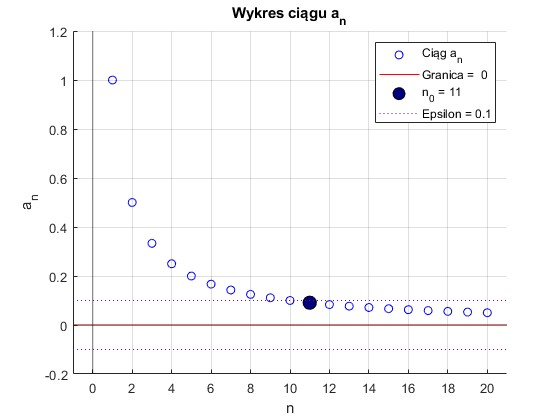
\includegraphics[width=0.8\textwidth]{Ciag_an.jpg}
\end{figure}
\subsection{Ciąg $b_n$ }
\raggedright{\textit{\textbf{Wzór: }} $b_n=\frac{2n^{2}+3n+4}{4n^{2}+5n}$}\\
\raggedright{\textit{\textbf{Skrypt:}}}
\begin{verbatim}
syms n; % Definiowanie n jako zmienną symboliczną
bn = (2*n^2 + 3*n + 4) / (4*n^2 + 5*n); % Wyrażenie ciągu

% Obliczenie granicy ciągu
limit_bn = limit(bn, n, inf);
limit_text = ['Granica = ', char(limit_bn)];

% Tworzenie wektora liczb naturalnych do wykresu
n_wartosc = 1:20; 

% Zapytanie użytkownika o epsilon
epsilon = input('Podaj epsilon > 0: ');

% Obliczenie wartości ciągu dla liczb naturalnych
bn_wartosc = (2*n_wartosc.^2 + 3*n_wartosc + 4) ./ (4*n_wartosc.^2 + 5*n_wartosc);

% Tworzenie wykresu
figure;
hold on;

% Wykres ciągu b_n
plot(n_wartosc, bn_wartosc, 'bo'); % Ciąg jako niebieskie kropki
plot([-1, 21], [limit_bn, limit_bn], 'r-'); % Granica jako czerwona linia ciągła

% Obliczenie n0 dla zadanego epsilon
n0_index = find(abs(bn_wartosc - limit_bn) < epsilon, 1);
n0 = n_wartosc(n0_index);

% Rysowanie n0 na wykresie
plot(n0, subs(bn, n, n0), 'ko', 'MarkerSize', 10, 'MarkerFaceColor', [0, 0, 0.5]); 
% Granatowa kropka na wykresie

% Rysowanie linii poziomej na wartości epsilon od granicy
plot([-1, 21], [limit_bn + epsilon, limit_bn + epsilon], ':', 'Color', [0.5, 0, 0.5]); 
% Epsilon od góry, linia przerywana, kolor fioletowy
plot([-1, 21], [limit_bn - epsilon, limit_bn - epsilon], ':', 'Color', [0.5, 0, 0.5]); 
% Epsilon od dołu, linia przerywana, kolor fioletowy

xlabel('n');
ylabel('b_n');
title('Wykres ciągu b_n');
legend('Ciąg b_n', limit_text, ['n_0 = ', num2str(n0)], ['Epsilon = ', num2str(epsilon)], 
'AutoUpdate', 'off');
grid on;
axis([-1, 21, -0.2, 1.2]); % Przeskalowanie osi x od -1 do 21 oraz osi y od -0.2 do 1.2
% Dodanie linii osi x i y
line([-1, 21], [0, 0], 'Color', [0, 0, 0, 0.5]); % Linia osi x
line([0, 0], [-0.2, 1.2], 'Color', [0, 0, 0, 0.5]); % Linia osi y
hold off;

\end{verbatim}
\raggedright{\textit{\textbf{Przykładowe wywołanie dla $\epsilon = 0.1$}}}
\begin{figure}[H]
	\centering
	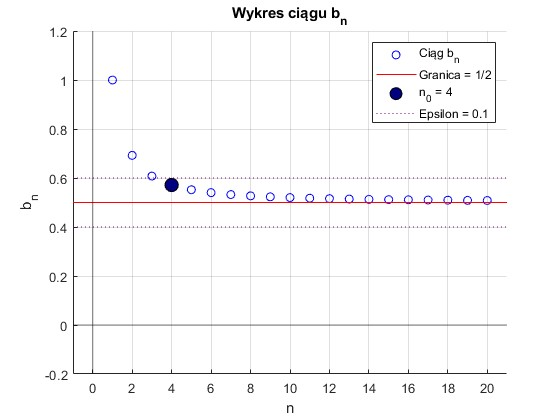
\includegraphics[width=0.8\textwidth]{Ciag_bn.jpg}
\end{figure}
\newpage
\subsection{Ciąg $c_n$ }
\raggedright{\textit{\textbf{Wzór: }}$c_n=\frac{1}{n+\log{(n+1)}}$}\\
\raggedright{\textit{\textbf{Skrypt:}}}
\begin{verbatim}
syms n; % Definiowanie n jako zmienną symboliczną
cn = 1 / (n + log(n + 1)); % Wyrażenie ciągu

% Obliczenie granicy ciągu
limit_cn = limit(cn, n, inf);
limit_text = ['Granica = ', char(limit_cn)];

% Tworzenie wektora liczb naturalnych do wykresu
n_wartosc = 1:20; 

% Zapytanie użytkownika o epsilon
epsilon = input('Podaj epsilon > 0: ');

% Obliczenie wartości ciągu dla liczb naturalnych
cn_wartosc = 1 ./ (n_wartosc + log(n_wartosc + 1));

% Tworzenie wykresu
figure;
hold on;

% Wykres ciągu c_n
plot(n_wartosc, cn_wartosc, 'bo'); % Ciąg jako niebieskie kropki
plot([-1, 21], [limit_cn, limit_cn], 'r-'); % Granica jako czerwona linia ciągła

% Obliczenie n0 dla zadanego epsilon
n0_index = find(abs(cn_wartosc - limit_cn) < epsilon, 1);
n0 = n_wartosc(n0_index);

% Rysowanie n0 na wykresie
plot(n0, subs(cn, n, n0), 'ko', 'MarkerSize', 10, 'MarkerFaceColor', [0, 0, 0.5]); 
% Granatowa kropka na wykresie

% Rysowanie linii poziomej na wartości epsilon od granicy
plot([-1, 21], [limit_cn + epsilon, limit_cn + epsilon], ':', 'Color', [0.5, 0, 0.5]); 
% Epsilon od góry, linia przerywana, kolor fioletowy
plot([-1, 21], [limit_cn - epsilon, limit_cn - epsilon], ':', 'Color', [0.5, 0, 0.5]); 
% Epsilon od dołu, linia przerywana, kolor fioletowy

xlabel('n');
ylabel('c_n');
title('Wykres ciągu c_n');
legend('Ciąg c_n', limit_text, ['n_0 = ', num2str(n0)], ['Epsilon = ', num2str(epsilon)], 
'AutoUpdate', 'off');
grid on;
axis([-1, 21, -0.2, 1.2]); % Przeskalowanie osi x od -1 do 21 oraz osi y od -0.2 do 1.2
% Dodanie linii osi x i y
line([-1, 21], [0, 0], 'Color', [0, 0, 0, 0.5]); % Linia osi x
line([0, 0], [-0.2, 1.2], 'Color', [0, 0, 0, 0.5]); % Linia osi y
hold off;

\end{verbatim}
\newpage
\raggedright{\textit{\textbf{Przykładowe wywołanie dla $\epsilon = 0.1$}}}
\begin{figure}[H]
	\centering
	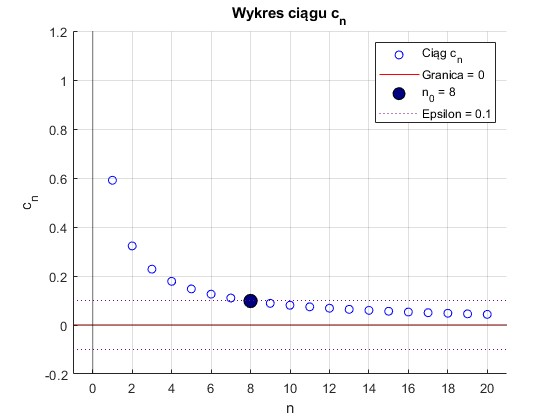
\includegraphics[width=0.8\textwidth]{Ciag_cn.jpg}
\end{figure}
\subsection{Ciąg $d_n$ }
\raggedright{\textit{\textbf{Wzór: }}$d_n = \frac{(3n^{2} + 5n - 1)}{\sqrt{n^{4} + 3n^{3} + 1}}$}\\
\raggedright{\textit{\textbf{Skrypt:}}}
\begin{verbatim}
syms n; % Definiowanie n jako zmienną symboliczną
dn = (3*n^2 + 5*n - 1) / sqrt(n^4 + 3*n^3 + 1); % Wyrażenie ciągu

% Obliczenie granicy ciągu
limit_dn = limit(dn, n, inf);
limit_text = ['Granica = ', char(limit_dn)];

% Tworzenie wektora liczb naturalnych do wykresu
n_wartosc = 1:20; 

% Zapytanie użytkownika o epsilon
epsilon = input('Podaj epsilon > 0: ');

% Obliczenie wartości ciągu dla liczb naturalnych
dn_wartosc = (3*n_wartosc.^2 + 5*n_wartosc - 1) ./ sqrt(n_wartosc.^4 + 3*n_wartosc.^3 + 1);

% Tworzenie wykresu
figure;
hold on;

% Wykres ciągu d_n
plot(n_wartosc, dn_wartosc, 'bo'); % Ciąg jako niebieskie kropki
plot([-1, 21], [limit_dn, limit_dn], 'r-'); % Granica jako czerwona linia ciągła

% Obliczenie n0 dla zadanego epsilon
n0_index = find(abs(dn_wartosc - limit_dn) < epsilon, 1);
n0 = n_wartosc(n0_index);


% Rysowanie n0 na wykresie
plot(n0, subs(dn, n, n0), 'ko', 'MarkerSize', 10, 'MarkerFaceColor', [0, 0, 0.5]); 
% Granatowa kropka na wykresie

% Rysowanie linii poziomej na wartości epsilon od granicy
plot([-1, 21], [limit_dn + epsilon, limit_dn + epsilon], ':', 'Color', [0.5, 0, 0.5]); 
% Epsilon od góry, linia przerywana, kolor fioletowy
plot([-1, 21], [limit_dn - epsilon, limit_dn - epsilon], ':', 'Color', [0.5, 0, 0.5]); 
% Epsilon od dołu, linia przerywana, kolor fioletowy

xlabel('n');
ylabel('d_n');
title('Wykres ciągu d_n');
legend('Ciąg d_n', limit_text, ['n_0 = ', num2str(n0)], ['Epsilon = ', num2str(epsilon)], 
'AutoUpdate', 'off');
grid on;
axis([-1, 21, -0.2, 4]); % Przeskalowanie osi x od -1 do 21 oraz osi y od -0.2 do 4
% Dodanie linii osi x i y
line([-1, 21], [0, 0], 'Color', [0, 0, 0, 0.5]); % Linia osi x
line([0, 0], [-0.2, 4], 'Color', [0, 0, 0, 0.5]); % Linia osi y
hold off;

\end{verbatim}
\raggedright{\textit{\textbf{Przykładowe wywołanie dla $\epsilon = 0.1$}}}
\begin{figure}[H]
	\centering
	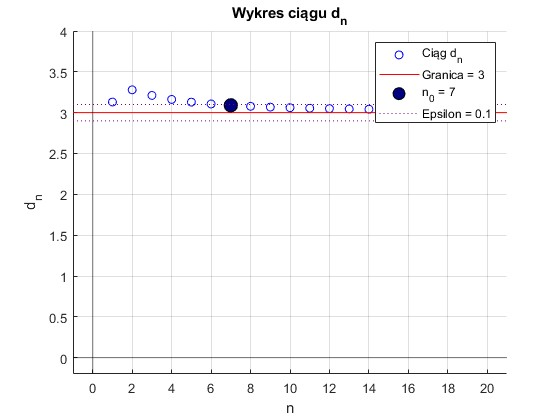
\includegraphics[width=0.8\textwidth]{Ciag_dn.jpg}
\end{figure}
\newpage
\subsection{Ciąg $e_n$ }
\raggedright{\textit{\textbf{Wzór: }}$e_n = \left( \frac{{n^2 + 3n + 2}}{{n^2 + 2n}} \right)^{2n+1}$}\\
\raggedright{\textit{\textbf{Skrypt:}}}
\begin{verbatim}
syms n; % Definiowanie n jako zmienną symboliczną
en = ((n^2 + 3*n + 2) / (n^2 + 2*n))^(2*n + 1); % Wyrażenie ciągu

% Obliczenie granicy ciągu
limit_en = limit(en, n, inf);
limit_text = ['Granica = ', char(limit_en)];

% Tworzenie wektora liczb naturalnych do wykresu
n_wartosc = 1:20; 

% Zapytanie użytkownika o epsilon
epsilon = input('Podaj epsilon > 0: ');

% Obliczenie wartości ciągu dla liczb naturalnych
en_wartosc = ((n_wartosc.^2 + 3*n_wartosc + 2) ./ (n_wartosc.^2 + 2*n_wartosc)).^(2*n_wartosc + 1);

% Tworzenie wykresu
figure;
hold on;

% Wykres ciągu e_n
plot(n_wartosc, en_wartosc, 'bo'); % Ciąg jako niebieskie kropki
plot([-1, 21], [limit_en, limit_en], 'r-'); % Granica jako czerwona linia ciągła

% Obliczenie n0 dla zadanego epsilon
n0_index = find(abs(en_wartosc - limit_en) < epsilon, 1);
n0 = n_wartosc(n0_index);

% Rysowanie n0 na wykresie
plot(n0, subs(en, n, n0), 'ko', 'MarkerSize', 10, 'MarkerFaceColor', [0, 0, 0.5]); 
% Granatowa kropka na wykresie

% Rysowanie linii poziomej na wartości epsilon od granicy
plot([-1, 21], [limit_en + epsilon, limit_en + epsilon], ':', 'Color', [0.5, 0, 0.5]); 
% Epsilon od góry, linia przerywana, kolor fioletowy
plot([-1, 21], [limit_en - epsilon, limit_en - epsilon], ':', 'Color', [0.5, 0, 0.5]); 
% Epsilon od dołu, linia przerywana, kolor fioletowy

xlabel('n');
ylabel('e_n');
title('Wykres ciągu e_n');
legend('Ciąg e_n', limit_text, ['n_0 = ', num2str(n0)], ['Epsilon = ', num2str(epsilon)], 
'AutoUpdate', 'off');
grid on;
axis([-0.2, 11, 4.2, 15]); % Przeskalowanie osi x od -0.2 do 11 oraz osi y od 4.2 do 15
% Dodanie linii osi x i y
line([-1, 21], [0, 0], 'Color', [0, 0, 0, 0.5]); % Linia osi x
line([0, 0], [4.2, 15], 'Color', [0, 0, 0, 0.5]); % Linia osi y
hold off;
	
\end{verbatim}
\newpage
\raggedright{\textit{\textbf{Przykładowe wywołanie dla $\epsilon = 0.1$}}}
\begin{figure}[H]
	\centering
	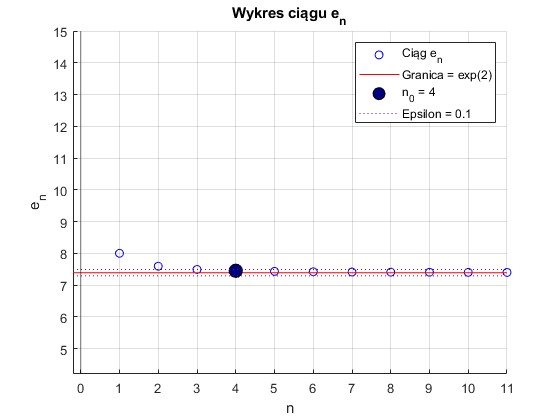
\includegraphics[width=0.8\textwidth]{Ciag_en.jpg}
\end{figure}
\subsection{Ciąg $f_n$ }
\raggedright{\textit{\textbf{Wzór: }}$f_n = \frac{{2^n + 3^n}}{{3^n + 4^n}}$}\\
\raggedright{\textit{\textbf{Skrypt:}}}
\begin{verbatim}
syms n; % Definiowanie n jako zmienną symboliczną
fn = (2^n + 3^n) / (3^n + 4^n); % Wyrażenie ciągu

% Obliczenie granicy ciągu
limit_fn = limit(fn, n, inf);
limit_text = ['Granica = ', char(limit_fn)];

% Tworzenie wektora liczb naturalnych do wykresu
n_wartosc = 1:20; 

% Zapytanie użytkownika o epsilon
epsilon = input('Podaj epsilon > 0: ');

% Obliczenie wartości ciągu dla liczb naturalnych
fn_wartosc = (2.^n_wartosc + 3.^n_wartosc) ./ (3.^n_wartosc + 4.^n_wartosc);

% Tworzenie wykresu
figure;
hold on;

% Wykres ciągu f_n
plot(n_wartosc, fn_wartosc, 'bo'); % Ciąg jako niebieskie kropki

% Obliczenie n0 dla zadanego epsilon
n0_index = find(abs(fn_wartosc - limit_fn) < epsilon, 1);
n0 = n_wartosc(n0_index);
% Rysowanie granicy na wykresie
plot([-1, 21], [limit_fn, limit_fn], 'r-'); % Granica jako czerwona linia ciągła

% Rysowanie n0 na wykresie
plot(n0, subs(fn, n, n0), 'ko', 'MarkerSize', 10, 'MarkerFaceColor', [0, 0, 0.5]); 
% Granatowa kropka na wykresie

% Rysowanie linii poziomej na wartości epsilon od granicy
plot([-1, 21], [limit_fn + epsilon, limit_fn + epsilon], ':', 'Color', [0.5, 0, 0.5]);
% Epsilon od góry, linia przerywana, kolor fioletowy
plot([-1, 21], [limit_fn - epsilon, limit_fn - epsilon], ':', 'Color', [0.5, 0, 0.5]); 
% Epsilon od dołu, linia przerywana, kolor fioletowy

xlabel('n');
ylabel('f_n');
title('Wykres ciągu f_n');
legend('Ciąg f_n', limit_text, ['n_0 = ', num2str(n0)], ['Epsilon = ', num2str(epsilon)], 
'AutoUpdate', 'off');
grid on;
axis([0, 21, -1, 2]); % Przeskalowanie osi x od 0 do 21 oraz osi y od -1 do 2
% Dodanie linii osi x i y
line([-1, 21], [0, 0], 'Color', [0, 0, 0, 0.5]); % Linia osi x
line([0, 0], [-1, 2], 'Color', [0, 0, 0, 0.5]); % Linia osi y
hold off;

\end{verbatim}
\raggedright{\textit{\textbf{Przykładowe wywołanie dla $\epsilon = 0.1$}}}
\begin{figure}[H]
	\centering
	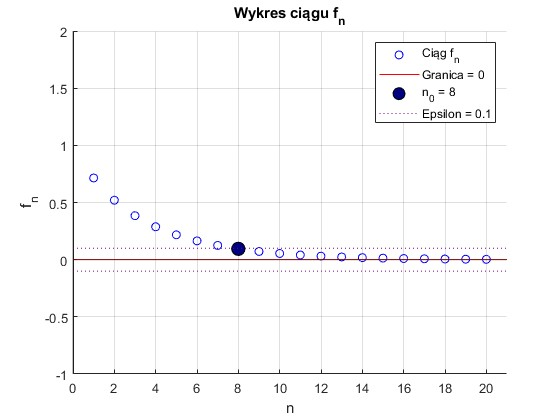
\includegraphics[width=0.8\textwidth]{Ciag_fn.jpg}
\end{figure}
\newpage
\subsection{Ciąg $g_n$ }
\raggedright{\textit{\textbf{Wzór: }}$g_n = \frac{{9^n n!}}{{(2n)!}}$}\\
\raggedright{\textit{\textbf{Skrypt:}}}
\begin{verbatim}
syms n; % Definiowanie n jako zmienną symboliczną
gn = (9^n * factorial(n)) / factorial(2*n); % Wyrażenie ciągu

% Obliczenie granicy ciągu
limit_gn = limit(gn, n, inf);
limit_text = ['Granica = ', char(limit_gn)];

% Tworzenie wektora liczb naturalnych do wykresu
n_wartosc = 1:20; 

% Zapytanie użytkownika o epsilon
epsilon = input('Podaj epsilon > 0: ');

% Obliczenie wartości ciągu dla liczb naturalnych
gn_wartosc = (9.^n_wartosc .* factorial(n_wartosc)) ./ factorial(2*n_wartosc);

% Tworzenie wykresu
figure;
hold on;

% Wykres ciągu g_n
plot(n_wartosc, gn_wartosc, 'bo'); % Ciąg jako niebieskie kropki

% Obliczenie n0 dla zadanego epsilon
n0_index = find(abs(gn_wartosc - limit_gn) < epsilon, 1);
n0 = n_wartosc(n0_index);

% Rysowanie granicy na wykresie
plot([-1, 21], [limit_gn, limit_gn], 'r-'); % Granica jako czerwona linia ciągła

% Rysowanie n0 na wykresie
plot(n0, subs(gn, n, n0), 'ko', 'MarkerSize', 10, 'MarkerFaceColor', [0, 0, 0.5]); 
% Granatowa kropka na wykresie

% Rysowanie linii poziomej na wartości epsilon od granicy
plot([-1, 21], [limit_gn + epsilon, limit_gn + epsilon], ':', 'Color', [0.5, 0, 0.5]); 
% Epsilon od góry, linia przerywana, kolor fioletowy
plot([-1, 21], [limit_gn - epsilon, limit_gn - epsilon], ':', 'Color', [0.5, 0, 0.5]); 
% Epsilon od dołu, linia przerywana, kolor fioletowy

xlabel('n');
ylabel('g_n');
title('Wykres ciągu g_n');
legend('Ciąg g_n', limit_text, ['n_0 = ', num2str(n0)], ['Epsilon = ', num2str(epsilon)], 
'AutoUpdate', 'off');
grid on;
axis([-1, 21, -0.5, 7]); % Przeskalowanie osi x od 0 do 21 oraz osi y od -0.5 do 7
% Dodanie linii osi x i y
line([-1, 21], [0, 0], 'Color', [0, 0, 0, 0.5]); % Linia osi x
line([0, 0], [-0.5, 7], 'Color', [0, 0, 0, 0.5]); % Linia osi y
hold off;

\end{verbatim}
\newpage 
\raggedright{\textit{\textbf{Przykładowe wywołanie dla $\epsilon = 0.1$}}}
\begin{figure}[H]
	\centering
	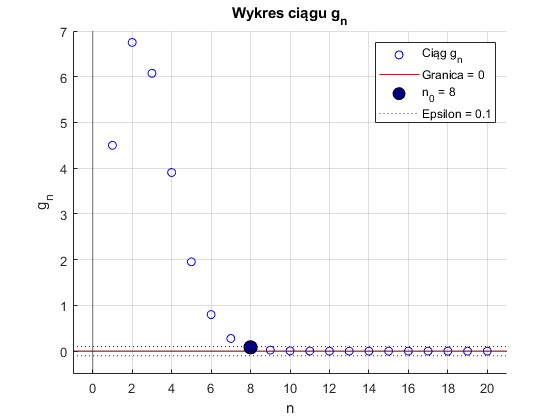
\includegraphics[width=0.8\textwidth]{Ciag_gn.jpg}
\end{figure}
\subsection{Ciąg $h_n$ }
\raggedright{\textit{\textbf{Wzór: }}$h_n = \frac{{n - \sin(3n)}}{{2n + \sin(4n)}}$}\\
\raggedright{\textit{\textbf{Skrypt:}}}
\begin{verbatim}
syms n; % Definiowanie n jako zmienną symboliczną
hn = (n - sin(3*n)) / (2*n + sin(4*n)); % Wyrażenie ciągu

% Obliczenie granicy ciągu
limit_hn = limit(hn, n, inf);
limit_text = ['Granica = ', char(limit_hn)];

% Tworzenie wektora liczb naturalnych do wykresu
n_wartosc = 1:20; 

% Zapytanie użytkownika o epsilon
epsilon = input('Podaj epsilon > 0: ');

% Obliczenie wartości ciągu dla liczb naturalnych
hn_wartosc = (n_wartosc - sin(3*n_wartosc)) ./ (2*n_wartosc + sin(4*n_wartosc));

% Tworzenie wykresu
figure;
hold on;

% Wykres ciągu h_n
plot(n_wartosc, hn_wartosc, 'bo'); % Ciąg jako niebieskie kropki

% Obliczenie n0 dla zadanego epsilon
n0_index = find(abs(hn_wartosc - limit_hn) < epsilon, 1);
n0 = n_wartosc(n0_index);

% Rysowanie granicy na wykresie
plot([-1, 21], [limit_hn, limit_hn], 'r-'); % Granica jako czerwona linia ciągła

% Rysowanie n0 na wykresie
plot(n0, subs(hn, n, n0), 'ko', 'MarkerSize', 10, 'MarkerFaceColor', [0, 0, 0.5]); 
% Granatowa kropka na wykresie

% Rysowanie linii poziomej na wartości epsilon od granicy
plot([-1, 21], [limit_hn + epsilon, limit_hn + epsilon], ':', 'Color', [0.5, 0, 0.5]); 
% Epsilon od góry, linia przerywana, kolor fioletowy
plot([-1, 21], [limit_hn - epsilon, limit_hn - epsilon], ':', 'Color', [0.5, 0, 0.5]); 
% Epsilon od dołu, linia przerywana, kolor fioletowy

xlabel('n');
ylabel('h_n');
title('Wykres ciągu h_n');
legend('Ciąg h_n', limit_text, ['n_0 = ', num2str(n0)], ['Epsilon = ', num2str(epsilon)], 
'AutoUpdate', 'off');
grid on;
axis([-1, 21, -1, 2]); % Przeskalowanie osi x od 0 do 21 oraz osi y od -1 do 2
% Dodanie linii osi x i y
line([-1, 21], [0, 0], 'Color', [0, 0, 0, 0.5]); % Linia osi x
line([0, 0], [-1, 2], 'Color', [0, 0, 0, 0.5]); % Linia osi y
hold off;

\end{verbatim}
\raggedright{\textit{\textbf{Przykładowe wywołanie dla $\epsilon = 0.1$}}}
\begin{figure}[H]
	\centering
	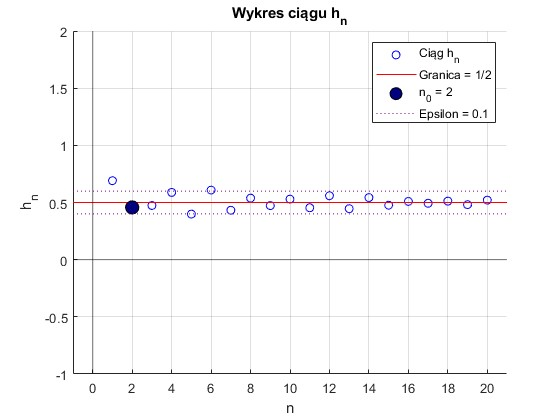
\includegraphics[width=0.8\textwidth]{Ciag_hn.jpg}
\end{figure}
\newpage
\section*{Źródła pomocnicze}
\patchcmd{\thebibliography}{\section*{\refname}}{}{}{}
\begin{thebibliography}{2}
	\bibitem{label1} 
	\href{https://staff.uz.zgora.pl/esylwest/pliki/Wyk3_mat_ET.pdf}{uz.zgora.pl}
	\bibitem{label2} 
	\href{https://ch.mathworks.com/help/matlab/index.html?s_tid=hc_panel}{mathworks.com}

\end{thebibliography}
\end{document}
